Посмотрим на поведение характеристик при фиксированных параметрах построения графов, но с варьирующимися параметрами распределений.\\

\hspace*{-1cm}
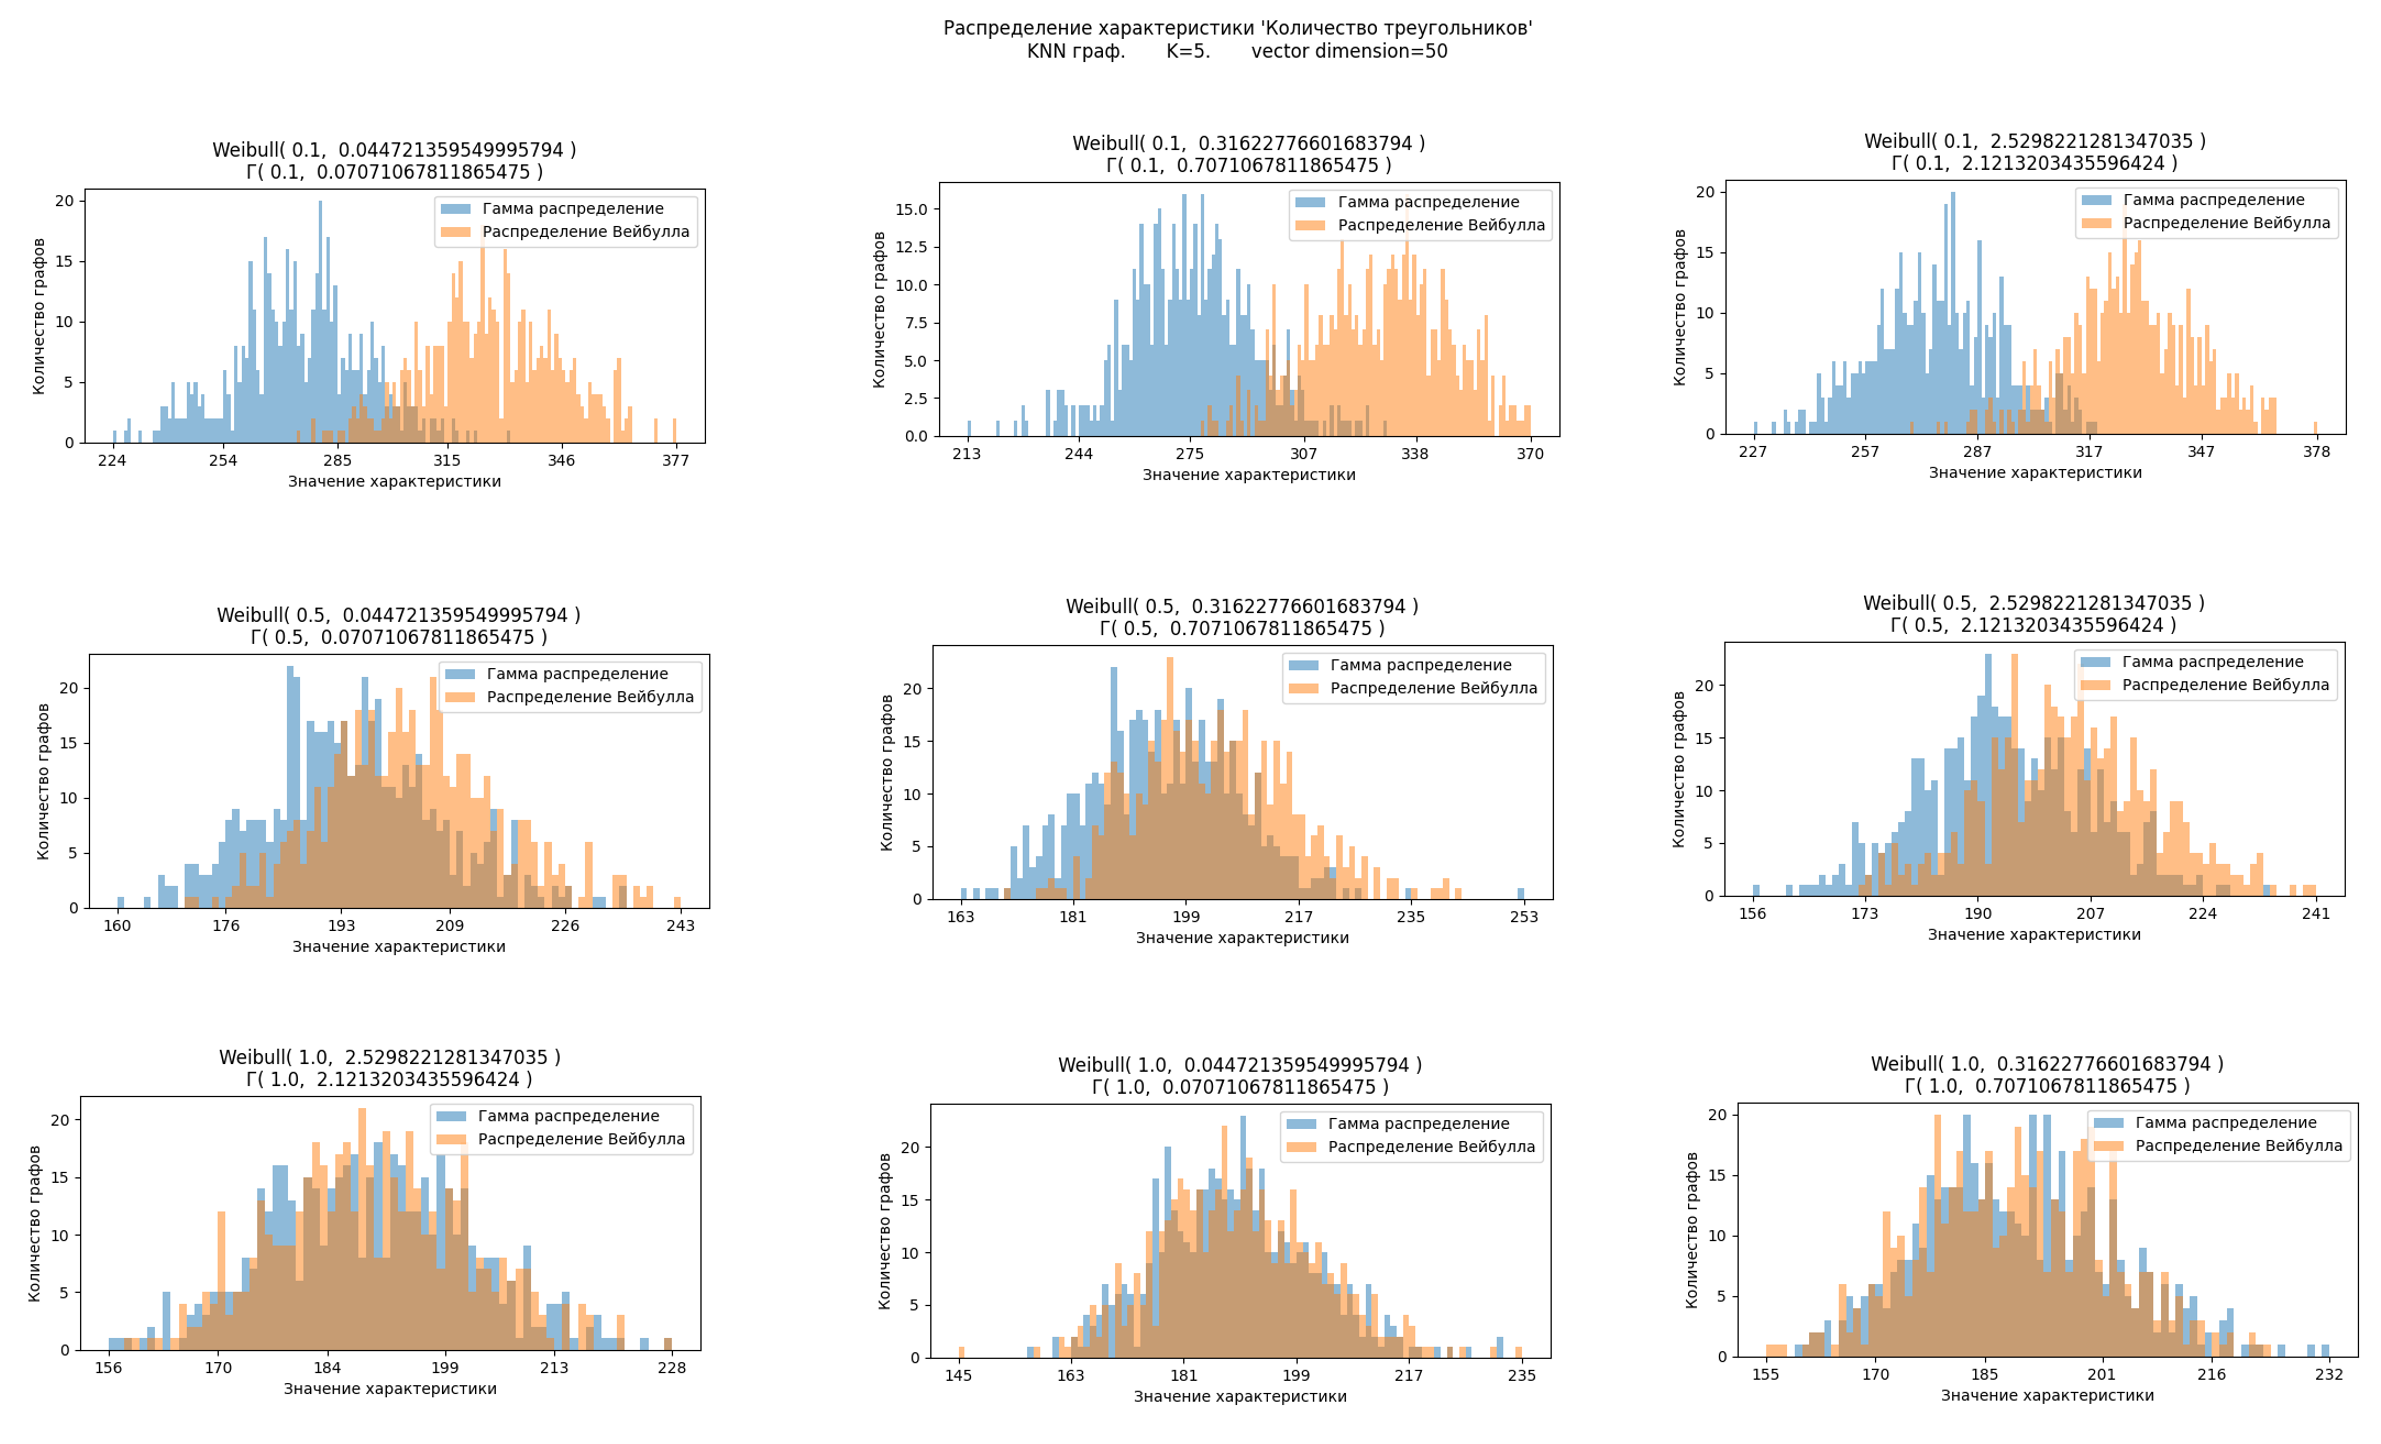
\includegraphics[width=1\textwidth]{Part-I_student-2/point 1_histogram_KNN.png}\\ 

\noindent\textbf{Вывод:} в зависимости от параметров распределений характеристика 'Количество треугольников' KNN графа может быть как хорошим признаком классификации (перекрытие гистограмм около нулевое), так и плохим (гистограммы практически идентичны).


\hspace*{-1cm}
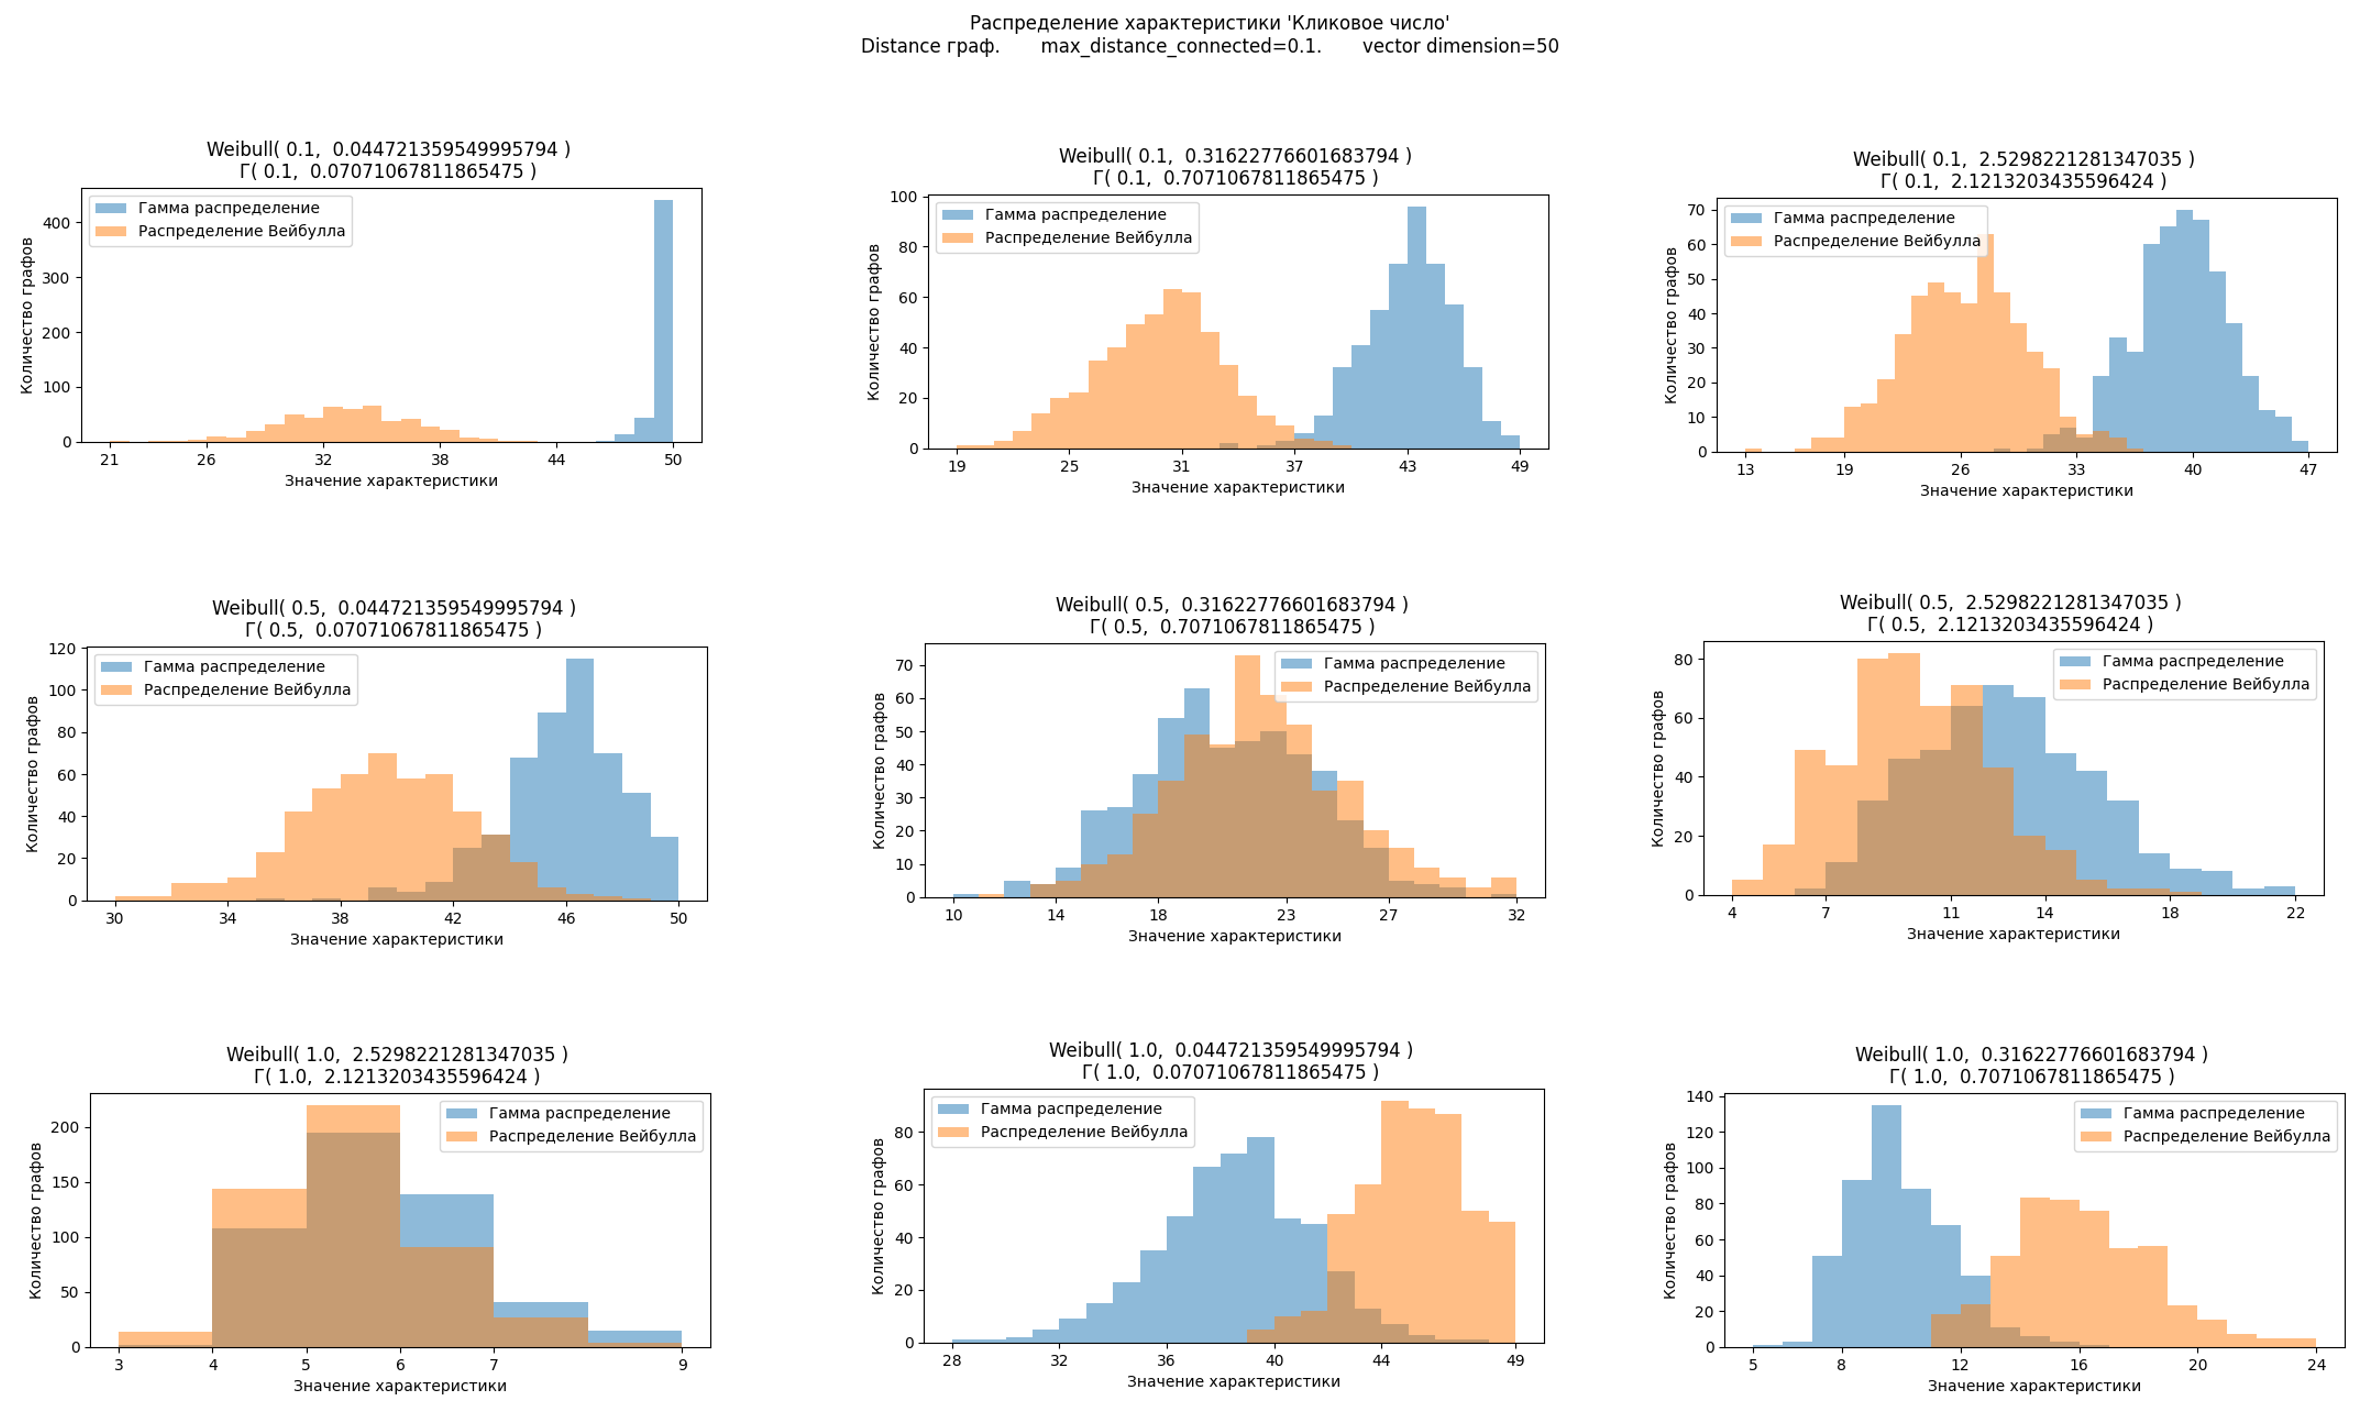
\includegraphics[width=1\textwidth]{Part-I_student-2/point 1_histogram_Dist.png}\\ 

\noindent\textbf{Вывод:} в зависимости от параметров распределений характеристика 'Кликовое число' Distance графа может быть как \textbf{очень хорошим} признаком классификации (перекрытие гистограмм нулевое), так и плохим (гистограммы практически идентичны).